%!LW recipe=XeLaTeXmk

\documentclass[scheme=plain]{ctexbeamer}
\usepackage[T1]{fontenc}
\usepackage{fontawesome5}
\usepackage{mathtools}
\usepackage{tikz}
\usepackage{booktabs}
\usepackage{caption}
\usepackage{outlines}
\usepackage{graphicx}
\usepackage{float}
\usepackage{amsthm}
\usepackage{tabularray}
\usepackage{minted}
\usepackage{hyperref}
\usepackage{cleveref}
\usepackage{url}
\usepackage{xspace}
\usepackage{academicons}
\usepackage{pgfplots}
\usepackage{pgfgantt}
\usepackage{qrcode}
\usepackage{ninecolors}

\usetheme[
    progressbar=frametitle,
    numbering=fraction,
    subsectionpage=progressbar,
    titleformat title=smallcaps,
    titleformat subtitle=smallcaps,
    titleformat section=smallcaps,
    titleformat frame=smallcaps]{metropolis}

\setbeamercolor{palette primary}{bg=gray1}
\setbeamercolor{frametitle}{bg=black,fg=white}
\setbeamercolor{progress bar}{fg=black}

\usetikzlibrary{calc}
\setcounter{tocdepth}{1}

\makeatletter
\newlength{\frametitle@padding}
\setlength{\frametitle@padding}{2.2ex}
\newcommand{\frametitlestrut@start}{
  \rule{0pt}{\frametitle@padding +%
    \totalheightof{%
      \ifcsdef{frametitleformat}{\frametitleformat X}{X}%
    }%
  }%
}

\newcommand{\frametitlestrut@end}{
  \rule[-\frametitle@padding]{0pt}{\frametitle@padding}
}

\setbeamertemplate{frametitle}{
    \nointerlineskip%
    \begin{beamercolorbox}[%
        wd=\paperwidth,%
        sep=0pt,%
        leftskip=\frametitle@padding,%
        rightskip=\frametitle@padding,%
      ]{frametitle}%
    \frametitlestrut@start%
    \insertframetitle%
    \hfill%
    \nolinebreak%
    \frametitlestrut@end%
    \end{beamercolorbox}%
    \begin{tikzpicture}[remember picture,overlay]
        \coordinate (logo) at ([xshift=-1.8cm,yshift=-0.6cm]current page.north east);
        \node at (logo) {
\includegraphics[height=.1\textheight]{northeastern.eps}};
    \end{tikzpicture}
}
\makeatother


\setbeamertemplate{footline}{
    \hbox{%
    \begin{beamercolorbox}[wd=\paperwidth,ht=3ex,dp=1.5ex,leftskip=2ex,rightskip=2ex]{page footer}%
        \usebeamerfont{title in head/foot}%
        \hfill
        \begin{tblr}{
            width=.8\linewidth,
            colspec={X[l]X[c]X[r]}
        }
            \insertsectionhead{}
            &
            \ifx\insertsubsection\empty
            \else
            \insertsubsection{} 
            \fi
            &
            \insertframenumber{} / \inserttotalframenumber
        \end{tblr}
        \hfill{}
    \end{beamercolorbox}}%
}

\defbeamertemplate{section page}{my progressbar}{
  \centering
  \begin{minipage}{22em}
    \raggedright
    \usebeamercolor[fg]{section title}
    \usebeamerfont{section title}
    \insertsection\\[-1ex]
    \usebeamertemplate*{progress bar in section page}
    \par
    \ifx\insertsubsectionhead\@empty\else%
      \usebeamercolor[fg]{subsection title}%
      \usebeamerfont{subsection title}%
      \insertsubsectionhead
    \fi
  \end{minipage}
  \par
  \vspace{\baselineskip}
}
\setbeamertemplate{section page}[my progressbar]

\UseTblrLibrary{booktabs}
\graphicspath{ {./images/} }

\title{Compression for AGI}
\author{Yuxuan Lu}
\institute{Northeastern Human-Centered AI Lab}
\date{Nov. 3 2023}

\begin{document}

\maketitle

\begin{frame}{Takeaways}
    \begin{outline}
        \1 Generative models are \emph{Lossless} compressors
            \2 ``ChatGPT Is a Blurry JPEG of the Web''? No!
        \1 LLMs are \emph{State-of-the-Art} text compressors
            \2 comparing to deflate(gzip), Zstd, etc.
        \1 Re-think about the training objective of foundation models
    \end{outline}
\end{frame}

\begin{frame}{Table of Contents}
    \tableofcontents
\end{frame}

\section[Training process of LLMs]{Revisit the Training Process of LLMs}
\begin{frame}{Transformer: A Black Box}
  \begin{figure}
      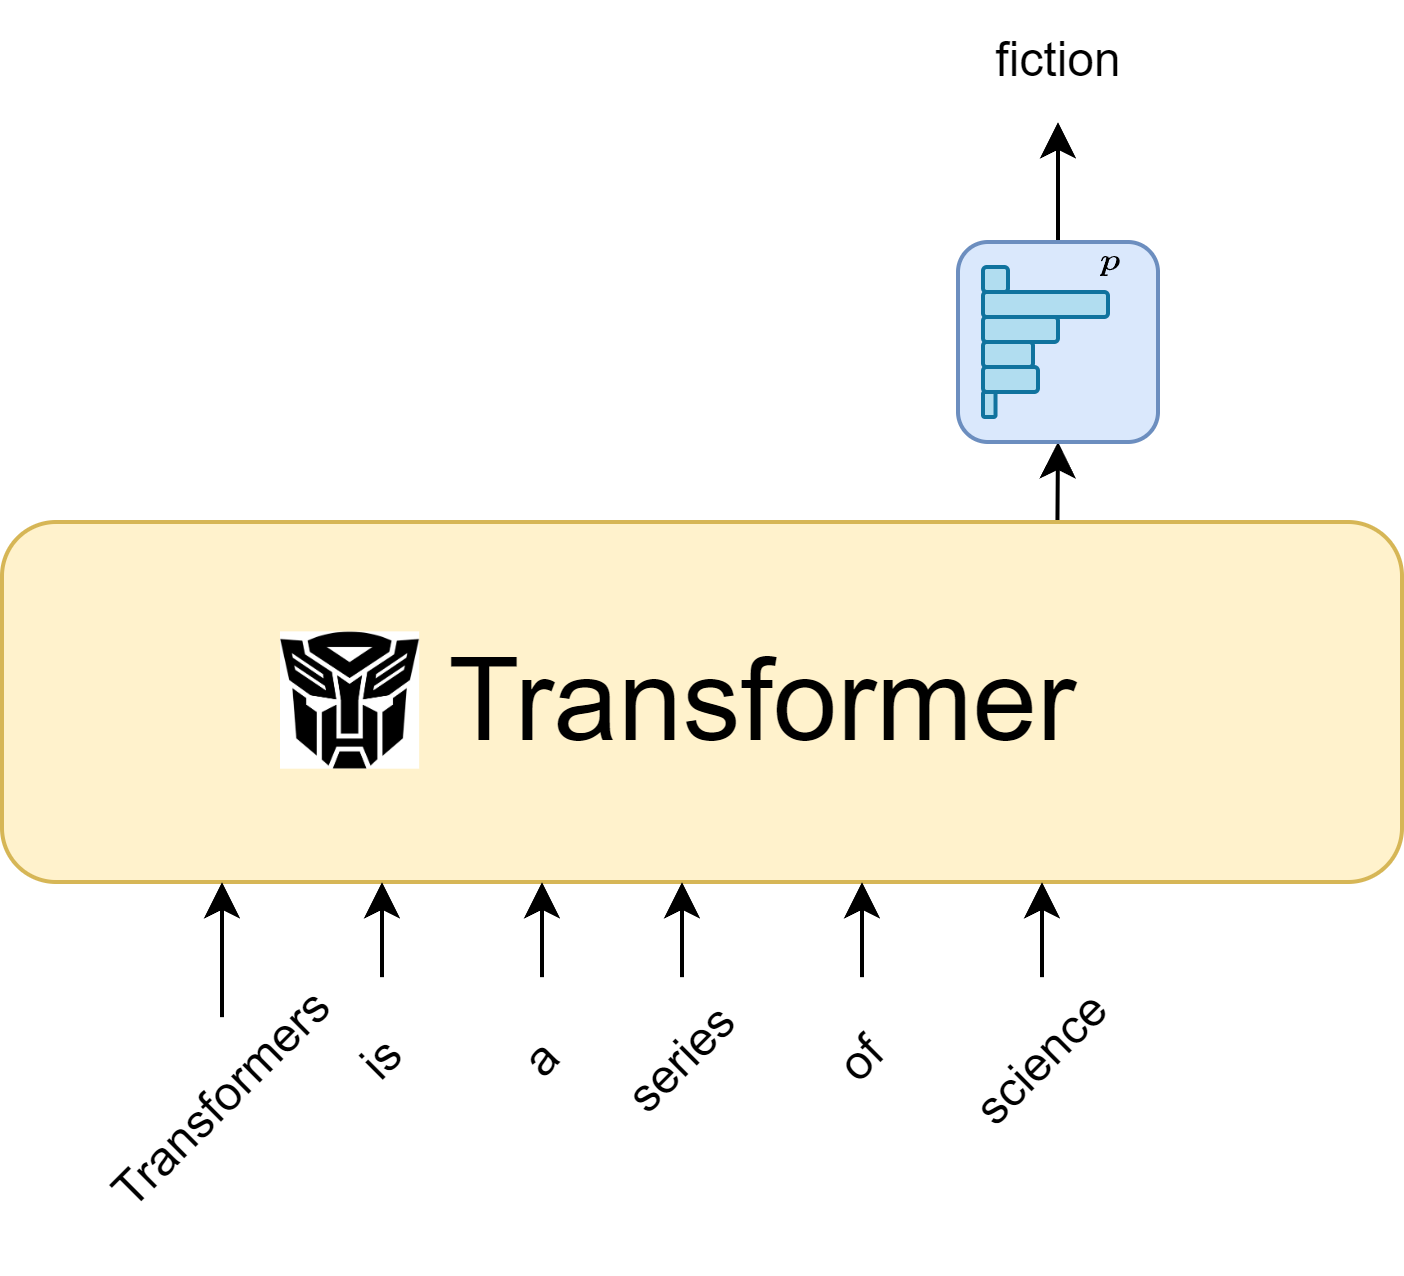
\includegraphics[width=.6\linewidth]{transformer_black_box.drawio.png}
      \caption[]{Transformer: A Black Box -- step 1}
  \end{figure}
\end{frame}
\begin{frame}{Transformer: A Black Box}
  \begin{figure}
      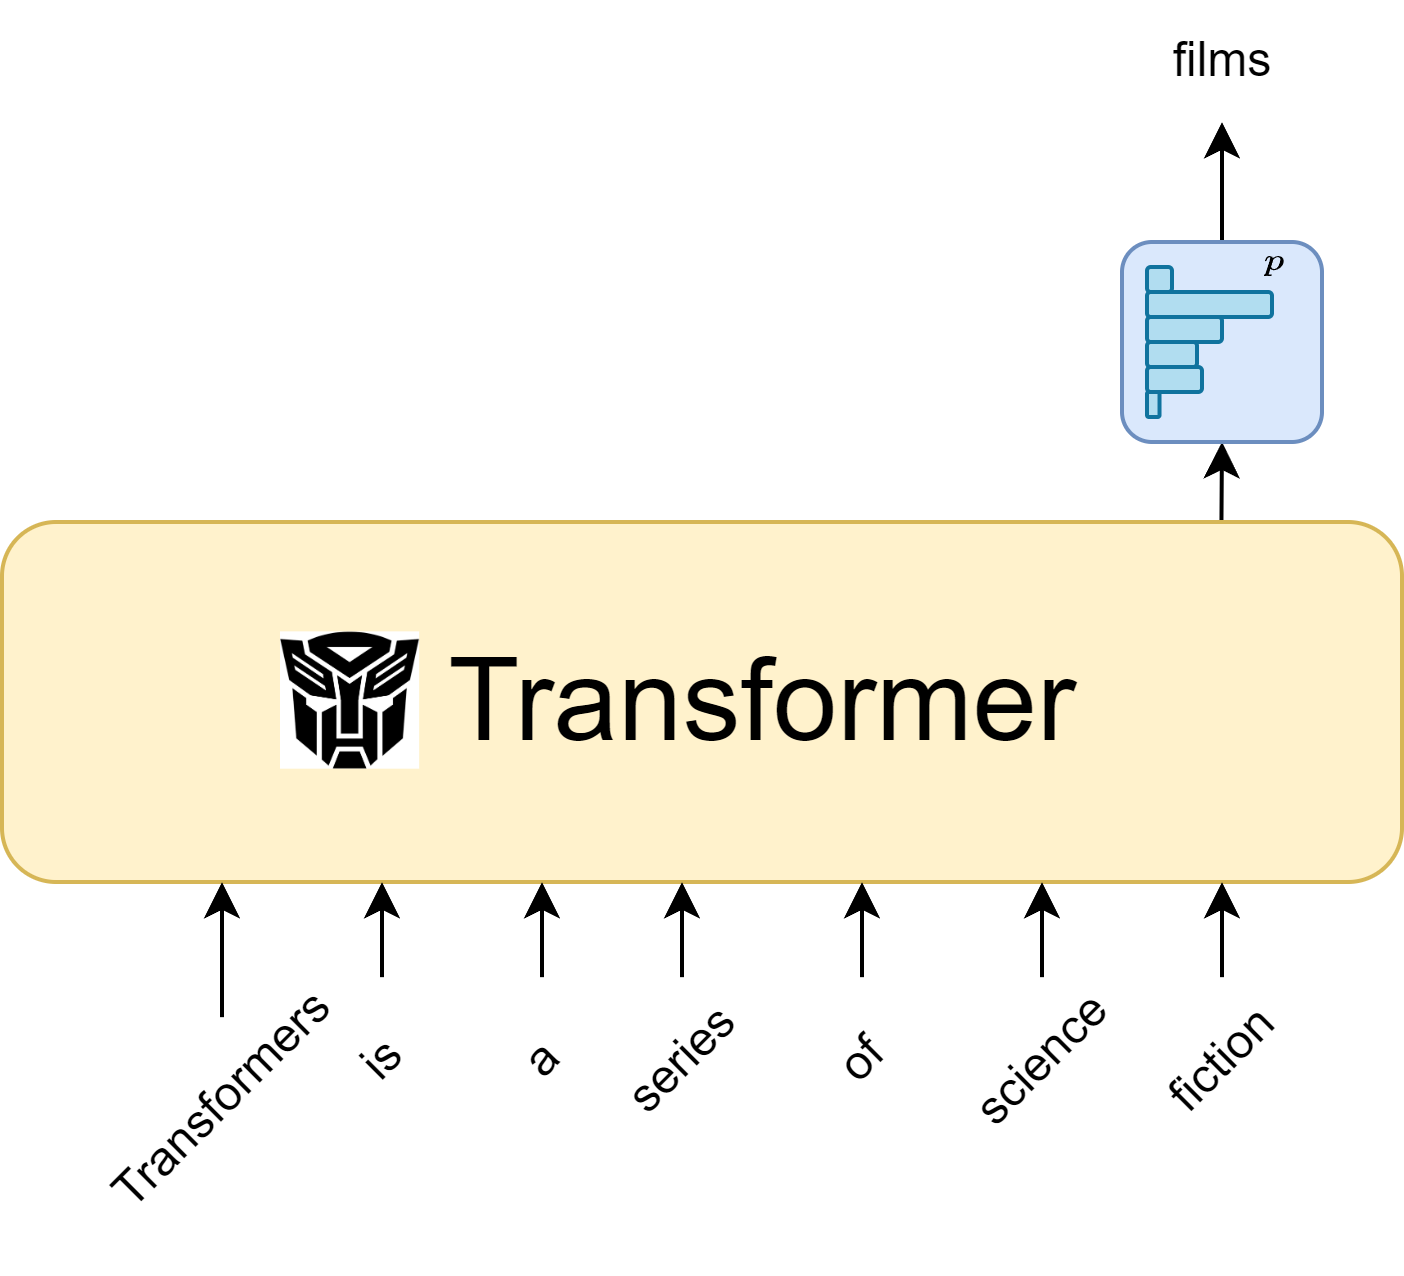
\includegraphics[width=.6\linewidth]{transformer_black_box_step_2.drawio.png}
      \caption[]{Transformer: A Black Box -- step 2}
  \end{figure}
\end{frame}
\begin{frame}{Transformer: A Black Box}
  \begin{figure}
      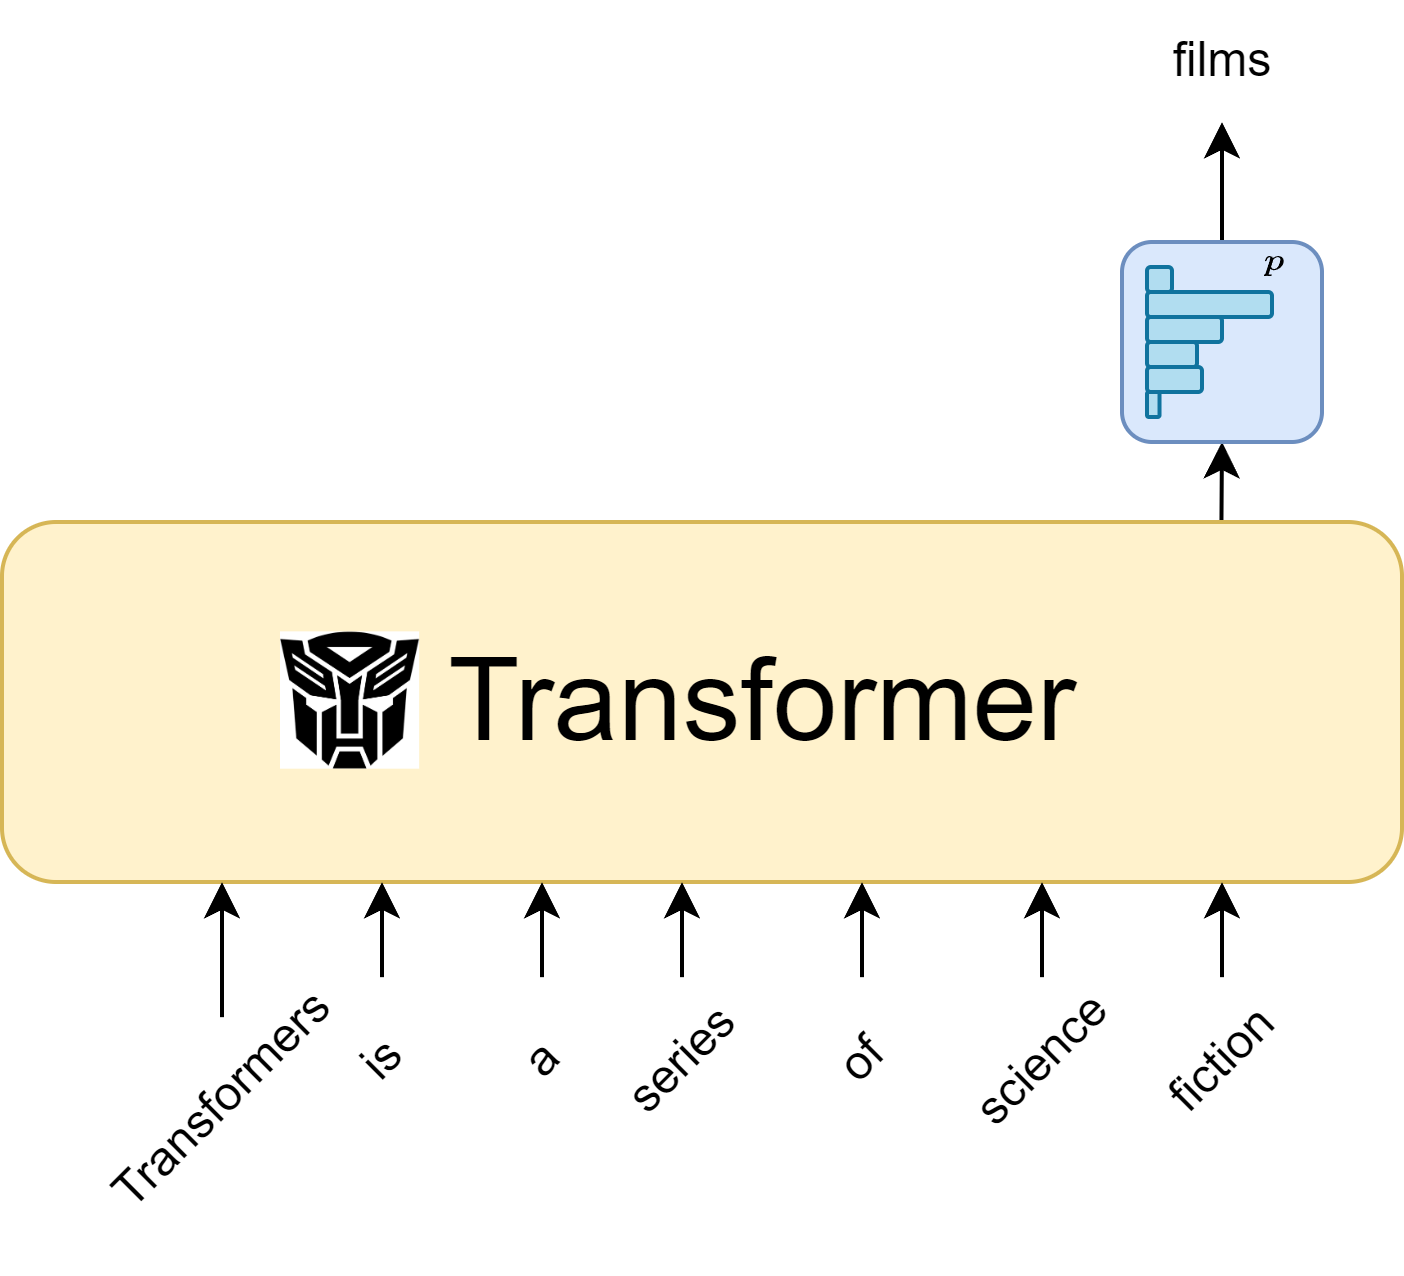
\includegraphics[width=.6\linewidth]{transformer_black_box_step_2.drawio.png}
      \caption[]{Transformer: A Black Box -- step 2}
  \end{figure}
\end{frame}
\begin{frame}{Transformer: A Black Box}
  \begin{figure}
      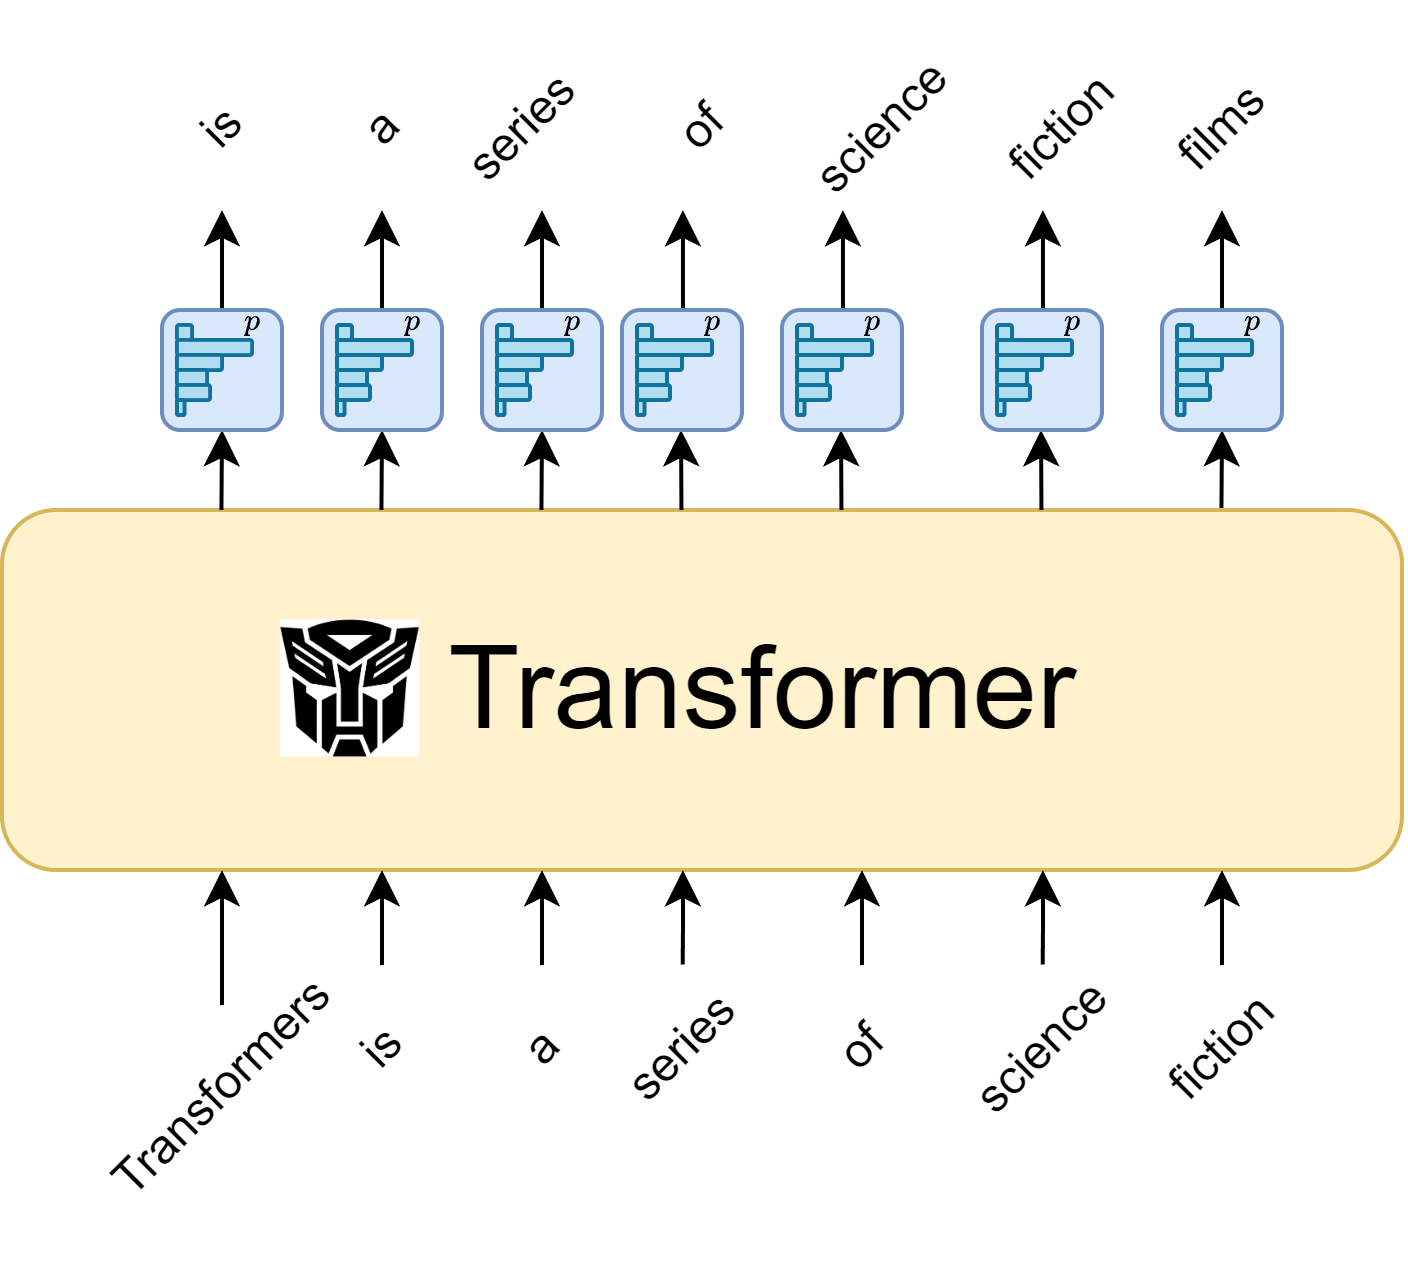
\includegraphics[width=.6\linewidth]{transformer_black_box_step_3.drawio.png}
      \caption[]{Transformer: A Black Box -- training}
  \end{figure}
\end{frame}
\begin{frame}{Transformer: A Black Box}
  \begin{outline}
    \1 We have a sequence: $ X = [x_1, x_2, \dots, x_n ] $
    \1 We put this sequence into LLM and get a sequence of probabilities:
      \2 $p_i = P(x_i | x_{<i})$
    \1 We want $p_i$ approachs $1$, so we minimize the following loss during pre-training:
      \2 $L = \sum_{i=1}^{n} - \log P(x_i | x_{<i})$
  \end{outline}
\end{frame}

\begin{frame}[standout]
  Questions?
\end{frame}

\section[Compressors]{What are compressors}
\begin{frame}{Compressor}
  \begin{outline}
    \1 Compressors aims to find a better (smaller) way to express the same thing
    \1 
  \end{outline}
\end{frame}

\section[LLMs as compressors]{Why are LLMs \emph{Lossless} compressors}

\begin{frame}{LLMs as compressors}
  \begin{outline}
    \1 Naturally, you would assume an LLM is a \emph{lossy} compressor
      \2 That turns trainig corpus to model parameters
      \2 For LLaMa, the training dataset is 5.6TB
      \2 And the 65 billion parameters takes about 130GB of storage
        \3 So 43x compression rate?
        \3 Lossy!
    \pause
    \1 Actually, LLaMa can compress the entire 5.6TB of training corpus to 397.3 GB losslessly
      \2 14x compression
      \2 Best text compressor: 8.7x compression
  \end{outline}
\end{frame}



\begin{frame}{LLMs as compressors}
  \begin{outline}
    \1 To compress the \emph{entire training corpus $\mathcal{C}$ losslessly}, we only need \emph{the CODE to train the models} and $\sum_{i \in \mathcal{C}} - \log P(x_i | x_{<i}) $ bits of imformation.
      \2 The result size (after compression) \emph{ISN'T} related the number of parameters!
      \pause
    \1 But, HOW?
  \end{outline}
\end{frame}

\begin{frame}{LLMs as compressors -- How}
  \begin{outline}
    \1 Imagine Alice is trying to send some text to Bob through a telephone wire
    \1 Sending the raw text is very expensive
      \2 too large
    \1 So Alice need to find a way to compress the data losslessly
    \1 Alice needs to encode the data to ``something''
    \1 Bob needs to decode the ``something'' back to data
    \1 So we need an ``encoding'' algorithm and a ``decoding'' algorithm
  \end{outline}
\end{frame}

\begin{frame}{LLMs as compressors -- Encoding}
  \begin{outline}
    \1 Let's say we have a vocabulary of \(\mathcal{V}\) (which should be defined in the training code), and we want to encode the first token \(x_1\).
    \pause
    \1 First, we initialize the model and fed it the training data
      \2 and we can get the probability distribution of the first token $p$ and an index $x_1 \in \mathcal{V}$
      \pause
    \1 With arithmetic encoding, we can encode the index $x_1$ with $-\log_2 p_{x_1}$ bits
      \2 Rather than $-\log_2 \frac{1}{|\mathcal{V}|}$ bits
      \pause
    \1 We send those $-\log_2 p_{x_1}$ bits to Bob
      \2 Let's call it $z_1$
      \pause
    \1 $\dots$ and update the model to minimize the loss, and repeat these steps for every data
  \end{outline}
\end{frame}

\begin{frame}{LLMs as compressors -- Decoding}
  \begin{outline}
    \1 Bob retrives the code for training the model
    \pause
    \1 And he can initialize the exact same model (with random seed defined in the code)
    \pause
    \1 So he will have the \emph{exact same distribution} $p$ for the first token
      \2 He then can decode the token with $p$ and $z_1$ with arithmetic decoding, get $x_1$
      \pause
    \1 And he will run the training loop to update the model with $x_1$
    \1 Note that the model parameters isn't transmitted through the phone wire
  \end{outline}
\end{frame}

\begin{frame}{LLMs as compressors -- Conclusion}
  \begin{outline}
    \1 By sharing the same code, Bob can initialize the same model as Alice's
    \1 With arithmetic encoding and decoding, bob can decode the token with the same probability distribution produced by the model and the encode transmitted from Alice
    \1 And by training at the same time, the model is always synced between Alice and Bob
  \end{outline}
\end{frame}

\begin{frame}{LLMs as compressors -- Conclusion}
  \begin{outline}
    % \1 In the above process, the model parameter is always synced between bob and alice
    \1 With arithmetic encoding, we can use fewer bits to encode something have a higher probability in a distribution.
      \2 If the distribution is uniform, $-\log_2 p_{x_i} = -\log_2 \frac{1}{|\mathcal{V}|}$, which is same as naive storage
      \2 And as the model is continually training, it can predict the next token with higher and higher probability.
    \1 Bob can re-construct the entire training corpus $\mathcal{C}$ with $\sum_{i \in \mathcal{C}} - \log P(x_i | x_{<i}) $ bits of information
      \2 Which is exactly the same with the sum of training loss on all tokens!
  \end{outline}
\end{frame}

\begin{frame}[standout]
  Questions?
\end{frame}

\section[LLM, compression and AGI]{Rethink the goal for foundation models}

\begin{frame}{Classic Chinese Room thought experiment}
  \begin{outline}
    \1 If a computer program translates English and Chinese using an oracle comprising all possible combinations of Chinese and English combinations.
      \2 Does it have understanding of translation?
    \pause
      \2 It has the \emph{least} understanding of translation
    \pause
    \1 What if it do it by a set of rules?
      \2 Tt have \emph{some} understanding of translation.
    \pause
    \1 If we can make the rule set smaller, it will generalise better.
  \end{outline}
\end{frame}

\begin{frame}{Lossy V.S. Lossless}
  \begin{outline}
    \1 ``Lossy'' compression means the model ``remembers'' everything in the training dataset
      \2 BAD generalization
    \1 ``Lossless'' compression means the model can better predict unseen data samples
      \2 Better compression means GOOD generalization
        \3 Because \emph{EVERY} example is unseen
  \end{outline}
\end{frame}

\begin{frame}{Target for Foundation Models}
  \begin{figure}
    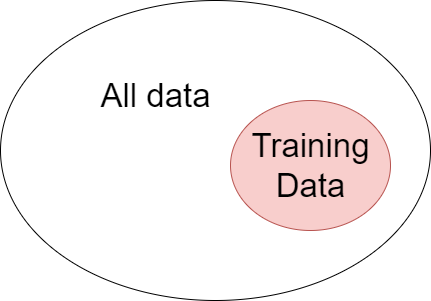
\includegraphics[width=.6\linewidth]{target_for_foundation_models.drawio.png}
    \caption{All data V.S. Training Data}
  \end{figure}
  \begin{outline}
    \1 For foundation models, what we want is good generalization ability
      \2 i.e. ability to generate or write \emph{UNSEEN} samples.
  \end{outline}
\end{frame}

\begin{frame}{``A recipe for perception''}
  \begin{outline}
    \0 A recipe for perception
      \1 Collet all useful perceptual information
      \1 Learn to compress it as best as possible with a powerful fundation model
        \2 Better architecture
        \2 Scale
        \2 Tool use
        \2 ...
  \end{outline}
\end{frame}


\begin{frame}{Conclusion}
  \begin{outline}
    \1 How LLM works
    \1 How LLM works as a compressor
      \2 And how should we use LLM
      \2 LLM isn't a search engine
    \1 How compressor generates intelligence
  \end{outline}
\end{frame}

\begin{frame}[standout]
  Questions?
\end{frame}


\end{document}


